\documentclass[aspectratio=169]{beamer}

\usetheme{Madrid}
\usecolortheme{default}
\setbeamertemplate{navigation symbols}{}

\usepackage[utf8]{inputenc}
\usepackage{tikz}
\usepackage{booktabs}
\usepackage{array}
\usepackage{amsmath}
\usepackage{svg}
\usepackage{fontawesome5}
\usetikzlibrary{arrows.meta, positioning, shapes.geometric, shapes.misc, calc, fit, backgrounds, decorations.pathreplacing}

\title{Introduction to Stream Processing}
\subtitle{From Batch Processing to Stateful Streaming Systems}
\author{Anh-Duc Le}
\date{\today}

% ---------------------------
% Styles
% ---------------------------
\tikzset{
    box/.style={
        draw,
        rounded corners,
        minimum width=2.2cm,
        minimum height=0.9cm,
        align=center
    },
    smallbox/.style={
        draw,
        rounded corners,
        minimum width=1.5cm,
        minimum height=0.65cm,
        align=center,
        font=\scriptsize
    },
    datastore/.style={
        cylinder,
        shape border rotate=90,
        draw,
        aspect=0.3,
        minimum height=1.1cm,
        minimum width=1.2cm,
        align=center
    },
    line/.style={-Latex, thick},
    dashedline/.style={-Latex, thick, dashed},
    barrier/.style={draw, diamond, aspect=2, inner sep=1pt, font=\scriptsize},
    watermark/.style={draw, cloud, cloud puffs=10, cloud ignores aspect, minimum width=1.8cm, minimum height=0.8cm, font=\scriptsize},
    note/.style={font=\scriptsize, align=left},
    tinylabel/.style={font=\tiny},
    every node/.style={font=\small}
}

\begin{document}

% -------------------------------------------------
\frame{\titlepage}

% -------------------------------------------------
\begin{frame}{Agenda}
\begin{enumerate}
    \item Why streaming now?
    \item Batch vs streaming: the mental model shift
    \item Core streaming concepts: event, stream, operator, state
    \item Time, windows, watermarks, and late data
    \item Flink state, checkpointing, and delivery guarantees
    \item Flink internals: barriers and backpressure
    \item End-to-end architecture: Kafka $\rightarrow$ Flink $\rightarrow$ Iceberg
    \item Practical guidance and Q\&A
\end{enumerate}
\end{frame}

% -------------------------------------------------
\begin{frame}{Who This Session Is For}
\begin{itemize}
    \item Data Engineers comfortable with batch systems such as Spark, Hive, SQL ETL, or Airflow orchestration
    \item Teams moving from periodic pipelines to low-latency or event-driven systems
    \item People who want to understand streaming as an engineering model, not just a tool
\end{itemize}

\vspace{0.4cm}
\textbf{Goal:} by the end, batch should feel like a special case of data processing, and streaming should feel operationally understandable rather than mysterious.
\end{frame}

% -------------------------------------------------
\begin{frame}{Why Streaming?}
\begin{itemize}
    \item Data is generated continuously: clicks, payments, logs, IoT, CDC, transactions
    \item The business often wants action before the batch window closes
    \item Lower latency unlocks:
    \begin{itemize}
        \item fraud detection
        \item operational alerting
        \item near-real-time dashboards
        \item dynamic pricing and personalization
        \item continuously updated data products
    \end{itemize}
\end{itemize}

\vspace{0.3cm}
\textbf{Core shift:} instead of storing all data first and computing later, compute continuously as data arrives.
\end{frame}

% -------------------------------------------------
\begin{frame}{Batch Processing Recap}
\begin{columns}[T]
\column{0.52\textwidth}
\textbf{Batch mental model}
\begin{itemize}
    \item Input is finite
    \item Run on schedule
    \item Recompute a result for a bounded slice
    \item Easy to reason about correctness
\end{itemize}

\column{0.48\textwidth}
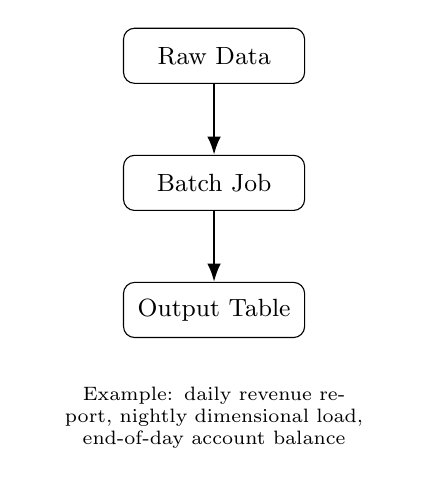
\begin{tikzpicture}[
    node distance=0.9cm,
    box/.style={
        draw,
        rounded corners,
        minimum width=2.3cm,
        minimum height=0.7cm,
        align=center,
        font=\small
    },
    line/.style={-Latex, thick},
    note/.style={
        align=center,
        font=\scriptsize,
        text width=4.5cm
    }
]

\node[box] (raw) {Raw Data};
\node[box, below=of raw] (job) {Batch Job};
\node[box, below=of job] (out) {Output Table};

\draw[line] (raw) -- (job);
\draw[line] (job) -- (out);

\node[note, below=0.5cm of out]
{Example: daily revenue report, nightly dimensional load, end-of-day account balance};

\end{tikzpicture}
\end{columns}

\vspace{0.3cm}
\textbf{Strong point:} excellent for large-volume recomputation over complete datasets.
\end{frame}

% -------------------------------------------------
\begin{frame}{Streaming Processing}
\begin{columns}[T]
\column{0.5\textwidth}
\textbf{Streaming mental model}
\begin{itemize}
    \item Input is unbounded
    \item Job is always on
    \item Results update incrementally
    \item State remembers history
\end{itemize}

\column{0.5\textwidth}
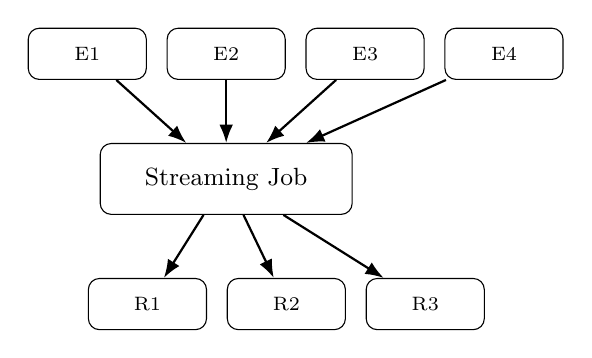
\begin{tikzpicture}[node distance=0.55cm]
\node[smallbox] (e1) {E1};
\node[smallbox, right=0.25cm of e1] (e2) {E2};
\node[smallbox, right=0.25cm of e2] (e3) {E3};
\node[smallbox, right=0.25cm of e3] (e4) {E4};

\node[box, below=0.8cm of e2, minimum width=3.2cm] (proc) {Streaming Job};
\node[smallbox, below=0.8cm of proc, xshift=-1.0cm] (r1) {R1};
\node[smallbox, right=0.25cm of r1] (r2) {R2};
\node[smallbox, right=0.25cm of r2] (r3) {R3};

\draw[line] (e1) -- (proc);
\draw[line] (e2) -- (proc);
\draw[line] (e3) -- (proc);
\draw[line] (e4) -- (proc);

\draw[line] (proc) -- (r1);
\draw[line] (proc) -- (r2);
\draw[line] (proc) -- (r3);
\end{tikzpicture}
\end{columns}

\vspace{0.3cm}
\textbf{Key point:} a streaming job does not wait for ``all the data'' because there is no final end to the stream.
\end{frame}

% -------------------------------------------------
\begin{frame}{Batch vs Streaming: The Mental Model Shift}
\begin{table}
\centering
\small
\begin{tabular}{>{\raggedright\arraybackslash}p{3.2cm} >{\raggedright\arraybackslash}p{4.0cm} >{\raggedright\arraybackslash}p{4.0cm}}
\toprule
Aspect & Batch & Streaming \\
\midrule
Dataset shape & Finite / bounded & Infinite / unbounded \\
Execution & Scheduled jobs & Long-running applications \\
Output & Complete snapshot & Incremental updates \\
Latency & Minutes to hours & Seconds to milliseconds \\
Memory of past & Usually in input tables & Maintained as state \\
Failure handling & Re-run batch & Recover state + resume \\
Time model & Often implicit & Must be explicit \\
\bottomrule
\end{tabular}
\end{table}

\vspace{0.3cm}
\textbf{Useful intuition:} batch is ``query over a bounded table,'' while streaming is ``continuous query over an ever-growing table.''
\end{frame}

% -------------------------------------------------
\begin{frame}{Core Concepts}
\begin{itemize}
    \item \textbf{Event}: one record, such as a payment, click, or CDC change
    \item \textbf{Stream}: ordered flow of events
    \item \textbf{Operator}: transformation, such as map, filter, join, aggregate
    \item \textbf{Key}: grouping dimension, such as customer\_id or account\_id
    \item \textbf{State}: data remembered between events
    \item \textbf{Window}: finite view over an unbounded stream
    \item \textbf{Watermark}: estimate of event-time progress
\end{itemize}
\end{frame}

% -------------------------------------------------
\begin{frame}{Events, Operators, and State}
\begin{center}
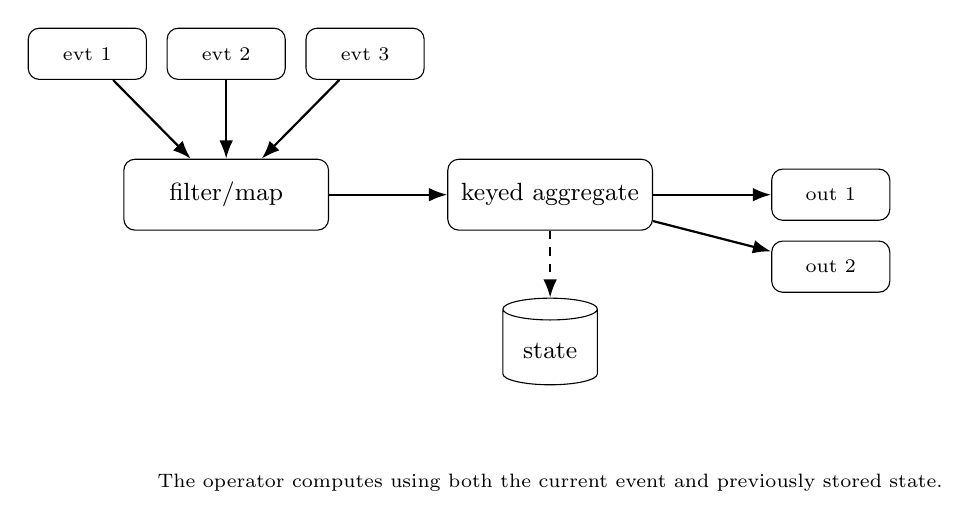
\begin{tikzpicture}[node distance=1.5cm]
\node[smallbox] (e1) {evt 1};
\node[smallbox, right=0.25cm of e1] (e2) {evt 2};
\node[smallbox, right=0.25cm of e2] (e3) {evt 3};

\node[box, below=1.0cm of e2, minimum width=2.6cm] (filter) {filter/map};
\node[box, right=1.5cm of filter, minimum width=2.6cm] (keyed) {keyed aggregate};
\node[datastore, below=0.85cm of keyed] (state) {state};

\node[smallbox, right=1.5cm of keyed] (out1) {out 1};
\node[smallbox, below=0.25cm of out1] (out2) {out 2};

\draw[line] (e1) -- (filter);
\draw[line] (e2) -- (filter);
\draw[line] (e3) -- (filter);

\draw[line] (filter) -- (keyed);
\draw[line] (keyed) -- (out1);
\draw[line] (keyed) -- (out2);
\draw[dashedline] (keyed) -- (state);

\node[note, below=1.0cm of state] {The operator computes using both the current event and previously stored state.};
\end{tikzpicture}
\end{center}
\end{frame}

% -------------------------------------------------
\begin{frame}{Stateful vs Stateless Processing}
\begin{columns}[T]
\column{0.5\textwidth}
\textbf{Stateless}
\begin{itemize}
    \item Output depends only on current event
    \item Example: parse JSON, filter invalid rows
    \item Easier to scale and reason about
\end{itemize}

\column{0.5\textwidth}
\textbf{Stateful}
\begin{itemize}
    \item Output depends on current + previous events
    \item Example: count per user, deduplication, sessionization, joins
    \item Requires persistence and recovery strategy
\end{itemize}
\end{columns}

\vspace{0.4cm}
\textbf{Streaming becomes powerful when state is involved.}
\end{frame}

% -------------------------------------------------
\begin{frame}{Keyed State vs Operator State}
\begin{columns}[T]
\column{0.48\textwidth}
\textbf{Keyed state = per entity}
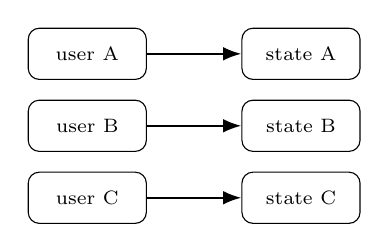
\begin{tikzpicture}[node distance=0.5cm]
\node[smallbox] (u1) {user A};
\node[smallbox, below=0.25cm of u1] (u2) {user B};
\node[smallbox, below=0.25cm of u2] (u3) {user C};

\node[smallbox, right=1.2cm of u1] (s1) {state A};
\node[smallbox, right=1.2cm of u2] (s2) {state B};
\node[smallbox, right=1.2cm of u3] (s3) {state C};

\draw[line] (u1) -- (s1);
\draw[line] (u2) -- (s2);
\draw[line] (u3) -- (s3);
\end{tikzpicture}

\vspace{0.2cm}
\begin{itemize}
    \item partitioned by key
    \item typical business logic
\end{itemize}

\column{0.48\textwidth}
\textbf{Operator state = per worker}
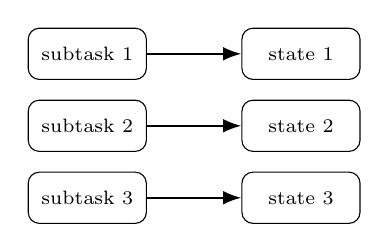
\begin{tikzpicture}[node distance=0.5cm]
\node[smallbox] (t1) {subtask 1};
\node[smallbox, below=0.25cm of t1] (t2) {subtask 2};
\node[smallbox, below=0.25cm of t2] (t3) {subtask 3};

\node[smallbox, right=1.2cm of t1] (o1) {state 1};
\node[smallbox, right=1.2cm of t2] (o2) {state 2};
\node[smallbox, right=1.2cm of t3] (o3) {state 3};

\draw[line] (t1) -- (o1);
\draw[line] (t2) -- (o2);
\draw[line] (t3) -- (o3);
\end{tikzpicture}

\vspace{0.2cm}
\begin{itemize}
    \item tied to operator instances
    \item common for sources / sinks
\end{itemize}
\end{columns}
\end{frame}

% -------------------------------------------------
\begin{frame}{Time in Streaming}
\begin{itemize}
    \item \textbf{Event time}: when the event actually happened in the real world
    \item \textbf{Processing time}: when the engine processed the event
    \item \textbf{Ingestion time}: when the system first observed the event
\end{itemize}

\vspace{0.3cm}
\textbf{Why this matters:}
\begin{itemize}
    \item network delays
    \item retries
    \item source buffering
    \item clock skew
    \item out-of-order delivery
\end{itemize}

\vspace{0.3cm}
If you care about business truth, event time usually matters more than processing time.
\end{frame}

% -------------------------------------------------
\begin{frame}{Event Time vs Processing Time Visualization}
\begin{center}
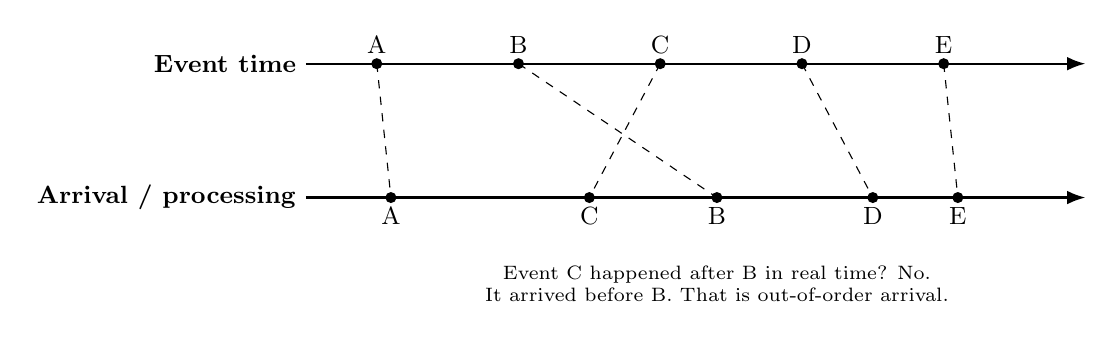
\begin{tikzpicture}[x=0.9cm,y=1cm]
% Event time
\draw[line] (0,2.5) -- (11,2.5);
\node[anchor=east] at (0,2.5) {\textbf{Event time}};

\foreach \x/\lbl in {1/A,3/B,5/C,7/D,9/E}{
    \fill (\x,2.5) circle (2pt);
    \node[above] at (\x,2.5) {\lbl};
}

% Processing time
\draw[line] (0,0.8) -- (11,0.8);
\node[anchor=east] at (0,0.8) {\textbf{Arrival / processing}};

\foreach \x/\lbl in {1.2/A,5.8/B,4.0/C,8.0/D,9.2/E}{
    \fill (\x,0.8) circle (2pt);
    \node[below] at (\x,0.8) {\lbl};
}

\draw[dashed] (1,2.5) -- (1.2,0.8);
\draw[dashed] (3,2.5) -- (5.8,0.8);
\draw[dashed] (5,2.5) -- (4.0,0.8);
\draw[dashed] (7,2.5) -- (8.0,0.8);
\draw[dashed] (9,2.5) -- (9.2,0.8);

\node[note, align=center] at (5.8,-0.3) {Event C happened after B in real time? No. \\ It arrived before B. That is out-of-order arrival.};
\end{tikzpicture}
\end{center}
\end{frame}

% -------------------------------------------------
\begin{frame}{Why Windows Exist}
\begin{itemize}
    \item A stream is unbounded, so many aggregates never naturally finish
    \item We create finite slices called windows to produce meaningful partial results
\end{itemize}

\vspace{0.3cm}
\textbf{Typical window types}
\begin{itemize}
    \item \textbf{Tumbling}: fixed-size, non-overlapping
    \item \textbf{Sliding}: fixed-size, overlapping
    \item \textbf{Session}: based on periods of inactivity
\end{itemize}
\end{frame}

% -------------------------------------------------
\begin{frame}{Window Types Visualization}
\begin{center}
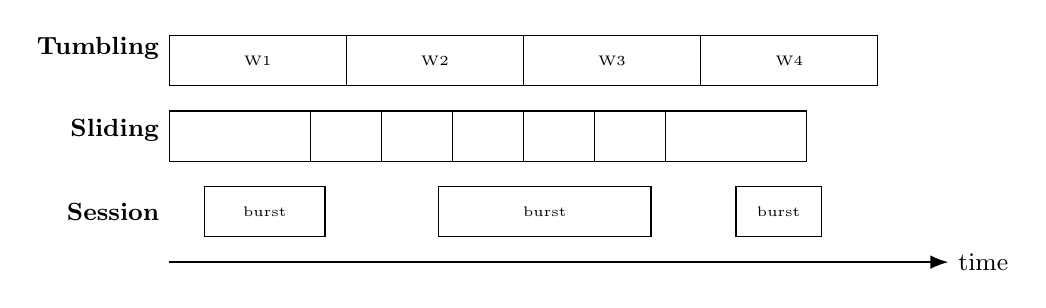
\begin{tikzpicture}[x=0.9cm,y=0.8cm]
\draw[line] (0,-0.6) -- (11,-0.6);
\node[anchor=west] at (11,-0.6) {time};

% Tumbling
\node[anchor=east] at (0,2.8) {\textbf{Tumbling}};
\draw (0,2.2) rectangle (2.5,3.0);
\draw (2.5,2.2) rectangle (5.0,3.0);
\draw (5.0,2.2) rectangle (7.5,3.0);
\draw (7.5,2.2) rectangle (10.0,3.0);
\node[tinylabel] at (1.25,2.6) {W1};
\node[tinylabel] at (3.75,2.6) {W2};
\node[tinylabel] at (6.25,2.6) {W3};
\node[tinylabel] at (8.75,2.6) {W4};

% Sliding
\node[anchor=east] at (0,1.5) {\textbf{Sliding}};
\draw (0,1.0) rectangle (3.0,1.8);
\draw (2.0,1.0) rectangle (5.0,1.8);
\draw (4.0,1.0) rectangle (7.0,1.8);
\draw (6.0,1.0) rectangle (9.0,1.8);

% Session
\node[anchor=east] at (0,0.2) {\textbf{Session}};
\draw (0.5,-0.2) rectangle (2.2,0.6);
\draw (3.8,-0.2) rectangle (6.8,0.6);
\draw (8.0,-0.2) rectangle (9.2,0.6);
\node[tinylabel] at (1.35,0.2) {burst};
\node[tinylabel] at (5.3,0.2) {burst};
\node[tinylabel] at (8.6,0.2) {burst};
\end{tikzpicture}
\end{center}
\end{frame}

% -------------------------------------------------
\begin{frame}{Non-Windowed Stream}
\begin{center}
\includesvg[width=0.88\textwidth]{svgs/non-windowed.svg}
\end{center}

\vspace{0.2cm}
\begin{itemize}
    \item This is an unbounded stream with no window boundaries.
    \item For many aggregations, this means the computation never naturally finishes.
    \item A result may keep updating forever unless we introduce a window or another cutoff rule.
\end{itemize}
\end{frame}

% -------------------------------------------------
% -------------------------------------------------
\begin{frame}{Non-Windowed Stream}
\begin{center}
\includesvg[width=0.5\textwidth]{svgs/non-windowed.svg}
\end{center}

\vspace{0.2cm}
\begin{itemize}
    \item This is an unbounded stream with no window boundaries.
    \item For many aggregations, this means the computation never naturally finishes.
    \item A result may keep updating forever unless we introduce a window or another cutoff rule.
\end{itemize}
\end{frame}

% -------------------------------------------------
\begin{frame}{Tumbling Windows}
\begin{center}
\includesvg[width=0.5\textwidth]{svgs/tumbling-windows.svg}
\end{center}

\vspace{0.2cm}
\begin{itemize}
    \item Tumbling windows are fixed-size and non-overlapping.
    \item Each event belongs to exactly one window.
    \item Good for periodic summaries such as revenue every 5 minutes or transactions per hour.
\end{itemize}
\end{frame}

% -------------------------------------------------
\begin{frame}{Sliding Windows}
\begin{center}
\includesvg[width=0.5\textwidth]{svgs/sliding-windows.svg}
\end{center}

\vspace{0.2cm}
\begin{itemize}
    \item Sliding windows have a window size and a slide interval.
    \item Windows overlap, so one event can belong to multiple windows.
    \item Useful for rolling metrics such as last 10 minutes, updated every 1 minute.
\end{itemize}
\end{frame}

% -------------------------------------------------
\begin{frame}{Session Windows}
\begin{center}
\includesvg[width=0.5\textwidth]{svgs/session-windows.svg}
\end{center}

\vspace{0.2cm}
\begin{itemize}
    \item Session windows are defined by activity separated by inactivity gaps.
    \item They are not fixed-size.
    \item Very useful for user behavior, clickstreams, or bursts of transactions.
\end{itemize}
\end{frame}

% -------------------------------------------------
\begin{frame}{Watermarks: The Practical Solution}
\begin{itemize}
    \item Streams may arrive out of order
    \item The engine needs a signal for when it is safe to finalize event-time windows
    \item A \textbf{watermark} is an estimate that says:
\end{itemize}

\begin{block}{}
``I do not expect future events with event time earlier than this watermark.''
\end{block}

\begin{itemize}
    \item Watermarks are heuristics, not guarantees from physics
    \item They let the system trade off latency vs completeness
\end{itemize}
\end{frame}

% -------------------------------------------------
\begin{frame}{Watermark + Late Data Visualization}
\begin{center}
\begin{tikzpicture}[x=0.9cm,y=0.9cm]

% Event-time axis
\draw[line] (0,0) -- (10,0);
\node[anchor=west] at (10,0) {event time};

% windows
\draw (0,0.4) rectangle (3,1.2);
\draw (3,0.4) rectangle (6,1.2);
\draw (6,0.4) rectangle (9,1.2);

\node[tinylabel] at (1.5,0.8) {[0,3)};
\node[tinylabel] at (4.5,0.8) {[3,6)};
\node[tinylabel] at (7.5,0.8) {[6,9)};

% arrival line
\draw[line] (0,-2.0) -- (10,-2.0);
\node[anchor=east] at (0,-2.0) {arrival};

% events
\foreach \x/\lbl in {1/A,2/B,3/C,4/D,5/E,6/F,7/G}{
    \fill (\x,-2.0) circle (2pt);
    \node[below] at (\x,-2.0) {\lbl};
}

% mapping lines
\draw[dashed] (1,-2.0) -- (1.2,0.4);
\draw[dashed] (2,-2.0) -- (2.4,0.4);
\draw[dashed] (3,-2.0) -- (4.5,0.4);
\draw[dashed] (4,-2.0) -- (5.4,0.4);
\draw[dashed] (5,-2.0) -- (7.0,0.4);
\draw[dashed, red] (6,-2.0) -- (2.0,0.4);
\draw[dashed] (7,-2.0) -- (7.8,0.4);

% watermark
\draw[very thick, blue, -Latex] (6.0,1.6) -- (6.0,-2.05);
\node[watermark, fill=white] at (6.0,2.0) {wm = 6};

\end{tikzpicture}
\end{center}

\vspace{0.2cm}

% explanation boxes BELOW (no overlap)
\begin{center}
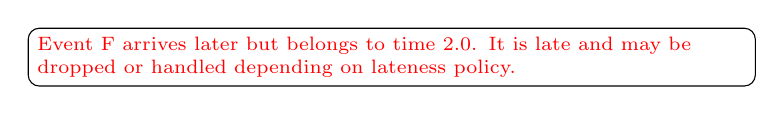
\begin{tikzpicture}

\vspace{0.15cm}

\node[
    draw,
    rounded corners,
    align=left,
    font=\scriptsize,
    text width=9cm,
    text=red
]
{
Event F arrives later but belongs to time 2.0. It is late and may be dropped or handled depending on lateness policy.
};
\end{tikzpicture}
\\When the watermark reaches 6, the window [3,6) is considered complete and can emit results.
\end{center}

\end{frame}

% -------------------------------------------------
\begin{frame}{What Can We Do With Late Data?}
\begin{itemize}
    \item \textbf{Drop it}: simplest, lowest latency
    \item \textbf{Allow lateness}: keep window open for a grace period
    \item \textbf{Emit updates}: correct previous results when late events arrive
    \item \textbf{Side output}: route late data for inspection or reprocessing
\end{itemize}

\vspace{0.4cm}
\textbf{Engineering trade-off:}
\begin{itemize}
    \item tighter watermark $\Rightarrow$ lower latency, more incomplete results
    \item looser watermark $\Rightarrow$ higher completeness, higher latency/state cost
\end{itemize}
\end{frame}

% -------------------------------------------------
\begin{frame}{Fault Tolerance in Streaming}
\begin{itemize}
    \item A long-running job must survive failures without losing correctness
    \item In Flink, correctness relies on \textbf{state snapshots} called checkpoints
    \item On failure, the job restarts from the latest successful snapshot
\end{itemize}

\vspace{0.3cm}
\textbf{Think of a checkpoint as:}
\begin{itemize}
    \item current operator state
    \item current source positions / offsets
    \item a consistent point across the dataflow
\end{itemize}
\end{frame}

% -------------------------------------------------
\begin{frame}{Checkpointing Visualization}
\begin{center}
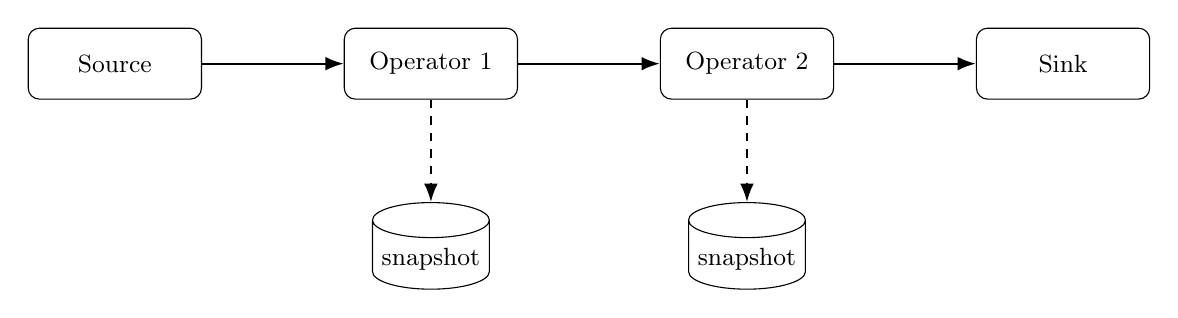
\begin{tikzpicture}[node distance=1.8cm]
\node[box] (src) {Source};
\node[box, right=of src] (op1) {Operator 1};
\node[box, right=of op1] (op2) {Operator 2};
\node[box, right=of op2] (sink) {Sink};

\draw[line] (src) -- (op1);
\draw[line] (op1) -- (op2);
\draw[line] (op2) -- (sink);

\node[datastore, below=1.3cm of op1] (cp1) {snapshot};
\node[datastore, below=1.3cm of op2] (cp2) {snapshot};

\draw[dashedline] (op1) -- (cp1);
\draw[dashedline] (op2) -- (cp2);

% \node[note, below=0.8cm of cp2, align=center] {};
A consistent snapshot lets Flink restore state and continue processing after failure.
\end{tikzpicture}
\end{center}
\end{frame}

% -------------------------------------------------
\begin{frame}{Processing Guarantees}
\begin{table}
\centering
\small
\begin{tabular}{>{\raggedright\arraybackslash}p{2.7cm} >{\raggedright\arraybackslash}p{7.5cm}}
\toprule
Guarantee & Meaning \\
\midrule
At-most-once & Fast, but records may be lost on failure \\
At-least-once & No loss, but duplicates may appear \\
Exactly-once & Each record affects result once, even across failures \\
\bottomrule
\end{tabular}
\end{table}

\vspace{0.3cm}
\textbf{Important nuance:}
\begin{itemize}
    \item Exactly-once is end-to-end only if the sink also participates correctly
    \item Engine guarantees alone are not enough if downstream writes are not atomic or idempotent
\end{itemize}
\end{frame}

% -------------------------------------------------
\begin{frame}{Flink Internals: Checkpoint Barriers}
\begin{center}
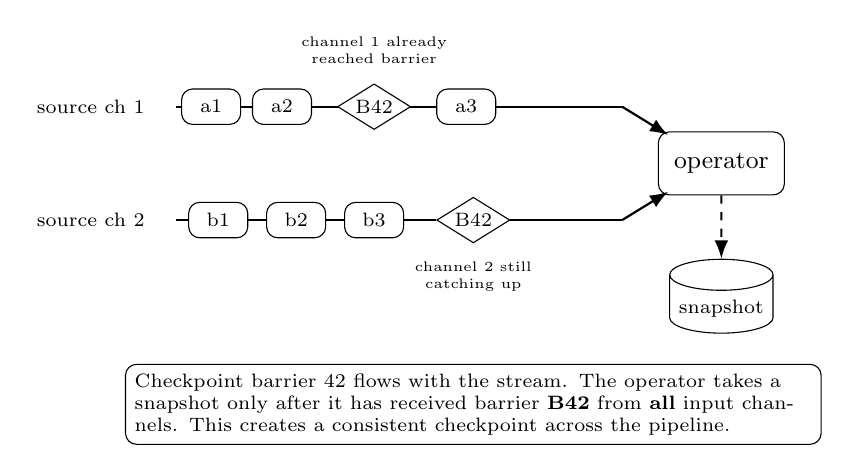
\begin{tikzpicture}[
    x=0.9cm,y=0.9cm,
    mybox/.style={
        draw,
        rounded corners,
        minimum width=1.6cm,
        minimum height=0.8cm,
        align=center,
        font=\small
    },
    mysmall/.style={
        draw,
        rounded corners,
        minimum width=0.75cm,
        minimum height=0.45cm,
        align=center,
        font=\scriptsize,
        fill=white
    },
    mybarrier/.style={
        draw,
        diamond,
        aspect=1.6,
        inner sep=1pt,
        font=\scriptsize,
        fill=white
    },
    mynote/.style={
        draw,
        rounded corners,
        align=left,
        font=\scriptsize,
        text width=8.6cm
    },
    myarrow/.style={-Latex, thick},
    mysnap/.style={
        cylinder,
        shape border rotate=90,
        draw,
        aspect=0.3,
        minimum height=0.9cm,
        minimum width=0.9cm,
        align=center,
        font=\scriptsize
    }
]

% labels
\node[anchor=east, font=\scriptsize] at (0.4,3.2) {source ch 1};
\node[anchor=east, font=\scriptsize] at (0.4,1.6) {source ch 2};

% top lane as separated segments
\draw[thick] (0.7,3.2) -- (0.82,3.2);
\draw[thick] (1.58,3.2) -- (1.82,3.2);
\draw[thick] (2.58,3.2) -- (3.02,3.2);
\draw[thick] (3.98,3.2) -- (4.42,3.2);
\draw[thick] (5.18,3.2) -- (7.0,3.2);
\draw[myarrow] (7.0,3.2) -- (7.65,2.8);

% bottom lane as separated segments
\draw[thick] (0.7,1.6) -- (0.92,1.6);
\draw[thick] (1.68,1.6) -- (2.02,1.6);
\draw[thick] (2.78,1.6) -- (3.12,1.6);
\draw[thick] (3.88,1.6) -- (4.38,1.6);
\draw[thick] (5.42,1.6) -- (7.0,1.6);
\draw[myarrow] (7.0,1.6) -- (7.65,2.0);

% top lane elements
\node[mysmall]   at (1.2,3.2) {a1};
\node[mysmall]   at (2.2,3.2) {a2};
\node[mybarrier] at (3.5,3.2) {B42};
\node[mysmall]   at (4.8,3.2) {a3};

% bottom lane elements
\node[mysmall]   at (1.3,1.6) {b1};
\node[mysmall]   at (2.4,1.6) {b2};
\node[mysmall]   at (3.5,1.6) {b3};
\node[mybarrier] at (4.9,1.6) {B42};

% annotations
\node[font=\tiny, align=center] at (3.5,4.0) {channel 1 already\\reached barrier};
\node[font=\tiny, align=center] at (4.9,0.8) {channel 2 still\\catching up};

% operator and snapshot
\node[mybox] (op) at (8.4,2.4) {operator};
\node[mysnap] (snap) at (8.4,0.35) {snapshot};
\draw[myarrow, dashed] (op) -- (snap);

% explanation
\node[mynote] at (4.9,-1.0)
{Checkpoint barrier 42 flows with the stream. The operator takes a snapshot only after it has received barrier \textbf{B42} from \textbf{all} input channels. This creates a consistent checkpoint across the pipeline.};

\end{tikzpicture}
\end{center}

\vspace{0.15cm}
\textbf{Idea:} barriers move with the data and align at multi-input operators.
\end{frame}

% -------------------------------------------------
\begin{frame}{Checkpoint Barrier Alignment Intuition}
\begin{itemize}
    \item Suppose an operator has multiple input channels
    \item Barrier 42 arrives on one channel before the others
    \item Flink temporarily buffers the early-arrived side so records do not cross the checkpoint boundary incorrectly
    \item Once all inputs have delivered barrier 42, the operator snapshot is consistent
\end{itemize}

\vspace{0.3cm}
\textbf{Why this matters:}
\begin{itemize}
    \item correctness under parallel execution
    \item consistent source offsets and operator state
    \item enables exactly-once semantics
\end{itemize}
\end{frame}

% -------------------------------------------------
\begin{frame}{Flink Internals: Backpressure Visualization}
\begin{center}
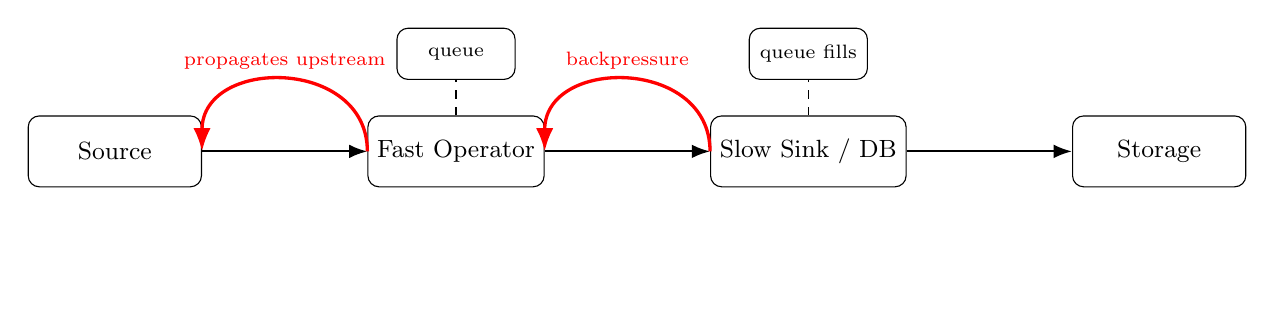
\begin{tikzpicture}[node distance=2.1cm]
\node[box] (src) {Source};
\node[box, right=of src] (fast) {Fast Operator};
\node[box, right=of fast] (slow) {Slow Sink / DB};
\node[box, right=of slow] (store) {Storage};

\draw[line] (src) -- (fast);
\draw[line] (fast) -- (slow);
\draw[line] (slow) -- (store);

% queue markers
\node[smallbox, above=0.45cm of fast] (q1) {queue};
\node[smallbox, above=0.45cm of slow] (q2) {queue fills};

\draw[dashed] (fast) -- (q1);
\draw[dashed] (slow) -- (q2);

% back arrows
\draw[red, very thick, -Latex] (slow.west) .. controls +(0,1.2) and +(0,1.2) .. node[above, font=\scriptsize] {backpressure} (fast.east);
\draw[red, very thick, -Latex] (fast.west) .. controls +(0,1.2) and +(0,1.2) .. node[above, font=\scriptsize] {propagates upstream} (src.east);

\node[note, below=1.0cm of fast, align=center] {};
\end{tikzpicture}
\begin{itemize}
    \item When a downstream operator cannot keep up, upstream tasks slow down too\\
    \item This is healthy signal propagation, but it increases latency and checkpoint times
\end{itemize}
\end{center}
\end{frame}

% -------------------------------------------------
\begin{frame}{Backpressure: What It Means Operationally}
\small
\begin{itemize}
    \item Usually caused by:
    \begin{itemize}
        \item slow external sink
        \item skewed key distribution
        \item expensive serialization or state access
        \item insufficient parallelism
    \end{itemize}
    \item Symptoms:
    \begin{itemize}
        \item growing end-to-end lag
        \item rising checkpoint duration
        \item busy or blocked tasks
        \item queue buildup and sink lag
    \end{itemize}
    \item Practical lesson: throughput is limited by the slowest stage
\end{itemize}
\end{frame}

% -------------------------------------------------
\begin{frame}{Backpressure: What It Means Operationally}
\small
\begin{itemize}
    \item Usually caused by:
    \begin{itemize}
        \item slow external sink
        \item skewed key distribution
        \item expensive serialization or state access
        \item insufficient parallelism
    \end{itemize}
    \item Symptoms:
    \begin{itemize}
        \item growing end-to-end lag
        \item rising checkpoint duration
        \item busy or blocked tasks
        \item queue buildup and sink lag
    \end{itemize}
    \item Practical lesson: throughput is limited by the slowest stage
\end{itemize}
\end{frame}

% -------------------------------------------------
\begin{frame}{End-to-End Architecture: Kafka $\rightarrow$ Flink $\rightarrow$ Iceberg}
\begin{center}
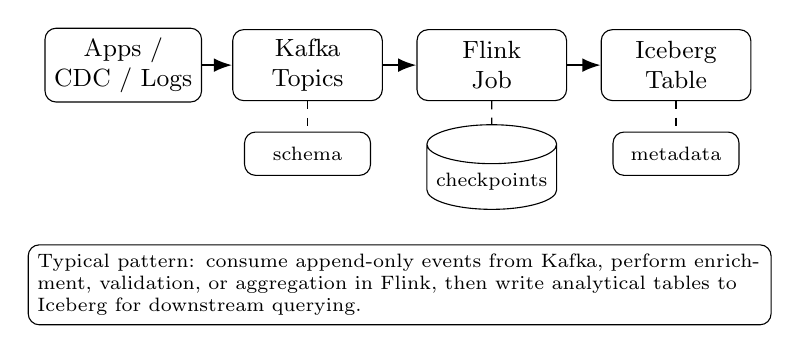
\begin{tikzpicture}[
    x=0.9cm,y=0.9cm,
    archbox/.style={
        draw,
        rounded corners,
        minimum width=1.9cm,
        minimum height=0.9cm,
        align=center,
        font=\small
    },
    archsmall/.style={
        draw,
        rounded corners,
        minimum width=1.6cm,
        minimum height=0.55cm,
        align=center,
        font=\scriptsize
    },
    archnote/.style={
        draw,
        rounded corners,
        text width=9.2cm,
        align=left,
        font=\scriptsize
    },
    archstore/.style={
        cylinder,
        shape border rotate=90,
        draw,
        aspect=0.3,
        minimum height=1.0cm,
        minimum width=1.0cm,
        align=center,
        font=\scriptsize
    },
    archline/.style={-Latex, thick}
]

% main flow
\node[archbox] (app) at (1.4,2.2) {Apps /\\ CDC / Logs};
\node[archbox] (kafka) at (4.0,2.2) {Kafka\\ Topics};
\node[archbox] (flink) at (6.6,2.2) {Flink\\ Job};
\node[archbox] (iceberg) at (9.2,2.2) {Iceberg\\ Table};

\draw[archline] (app) -- (kafka);
\draw[archline] (kafka) -- (flink);
\draw[archline] (flink) -- (iceberg);

% lower support row
\node[archsmall] (schema) at (4.0,0.95) {schema};
\node[archstore] (cp) at (6.6,0.55) {checkpoints};
\node[archsmall] (meta) at (9.2,0.95) {metadata};

\draw[dashed] (kafka) -- (schema);
\draw[dashed] (flink) -- (cp);
\draw[dashed] (iceberg) -- (meta);

% explanation box below
\node[archnote] at (5.3,-0.9)
{Typical pattern: consume append-only events from Kafka, perform enrichment, validation, or aggregation in Flink, then write analytical tables to Iceberg for downstream querying.};

\end{tikzpicture}
\end{center}
\end{frame}

% -------------------------------------------------
\begin{frame}{Architecture Detail: What Each Layer Does}
\begin{table}
\centering
\small
\begin{tabular}{>{\raggedright\arraybackslash}p{2.1cm} >{\raggedright\arraybackslash}p{8.2cm}}
\toprule
Layer & Responsibility \\
\midrule
Kafka & Durable event log, partitioning, replay, decoupling producers and consumers \\
Flink & Stateless + stateful processing, event-time logic, windowing, joins, enrichment, checkpointed recovery \\
Iceberg & Table abstraction on data lake, snapshots, partition evolution, analytics-friendly storage for batch and interactive engines \\
\bottomrule
\end{tabular}
\end{table}
\end{frame}

% -------------------------------------------------
\begin{frame}{Example Data Flow}
\begin{enumerate}
    \item Producer sends payment event into Kafka
    \item Flink consumes from topic partitions
    \item Job validates schema and filters bad records
    \item Job keys by account\_id or customer\_id
    \item Stateful logic calculates rolling totals or suspicious patterns
    \item Enriched or aggregated results are written to Iceberg
    \item BI, SQL engines, or ML jobs consume the Iceberg table
\end{enumerate}

\vspace{0.3cm}
\textbf{Why teams like this pattern:}
\begin{itemize}
    \item Kafka for event durability and replay
    \item Flink for low-latency logic
    \item Iceberg for reliable table consumption
\end{itemize}
\end{frame}

% -------------------------------------------------
\begin{frame}{Batch and Streaming Together, Not Opposed}
\begin{itemize}
    \item Streaming does not replace batch in all cases
    \item Instead:
    \begin{itemize}
        \item streaming handles low-latency, continuous updates
        \item batch handles large historical recomputation, model training, and backfills
    \end{itemize}
    \item Iceberg or lakehouse tables often become the meeting point between both worlds
\end{itemize}

\vspace{0.3cm}
\textbf{Good conceptual architecture model:}
\begin{itemize}
    \item Kafka = operational event log
    \item Flink = continuous compute engine
    \item Iceberg = durable analytical serving layer
\end{itemize}
\end{frame}

% -------------------------------------------------
\begin{frame}{When to Use Stateful Streaming}
\begin{itemize}
    \item Use stateful streaming when your logic depends on \textbf{history}
    
    \vspace{0.2cm}
    \textbf{Typical patterns:}
    \begin{itemize}
        \item Aggregation over time
        \begin{itemize}
            \item running totals, rolling averages
        \end{itemize}
        \item Entity-level tracking
        \begin{itemize}
            \item per user, account, device, session
        \end{itemize}
        \item Event correlation
        \begin{itemize}
            \item join streams, detect sequences, fraud patterns
        \end{itemize}
        \item Deduplication
        \begin{itemize}
            \item remember seen IDs or events
        \end{itemize}
    \end{itemize}

    \vspace{0.3cm}
    \textbf{Key signal:} you need to answer questions like
    \begin{block}{}
    ``What happened before this event?''
    \end{block}
\end{itemize}
\end{frame}

% -------------------------------------------------
\begin{frame}{When NOT to Use Stateful Streaming}
\begin{itemize}
    \item Do \textbf{not} use stateful streaming if your problem does not require memory

    \vspace{0.2cm}
    \textbf{Better alternatives:}
    \begin{itemize}
        \item Stateless streaming
        \begin{itemize}
            \item parsing, filtering, routing, enrichment via lookup
        \end{itemize}
        \item Batch processing
        \begin{itemize}
            \item large historical recomputation
            \item offline analytics or model training
        \end{itemize}
    \end{itemize}

    \vspace{0.3cm}
    \textbf{Warning signs:}
    \begin{itemize}
        \item ``We can recompute everything later anyway''
        \item ``Latency does not matter''
        \item ``State would grow unbounded without clear TTL''
    \end{itemize}

    \vspace{0.3cm}
    \textbf{Rule of thumb:}
    \begin{block}{}
    If you don’t need history, don’t introduce state.
    \end{block}
\end{itemize}
\end{frame}

% -------------------------------------------------
\begin{frame}{What Each Paradigm Can (and Cannot) Solve}
\small
\begin{tabular}{p{3cm} p{3.2cm} p{3.2cm} p{3.2cm}}
\toprule
 & Stateless Streaming & Stateful Streaming & Batch \\
\midrule
Latency & Low & Low & High \\
History awareness & No & Yes & Yes \\
Continuous results & Yes & Yes & No \\
Full recomputation & No & Hard & Yes \\
Complex joins & Limited & Yes & Yes \\
\midrule
Best for & Filtering, routing & Real-time logic & Historical analytics \\
\bottomrule
\end{tabular}

\vspace{0.4cm}

\textbf{Important:}
\begin{itemize}
    \item No single paradigm solves everything
    \item Most real systems combine:
    \begin{itemize}
        \item streaming for real-time
        \item batch for backfill and correctness
    \end{itemize}
\end{itemize}
\end{frame}

% -------------------------------------------------
\begin{frame}{Example Story: Fraud Detection}
\begin{itemize}
    \item Imagine detecting suspicious transactions in a banking system

    \vspace{0.2cm}
    \textbf{Stateless streaming fails:}
    \begin{itemize}
        \item each transaction is evaluated independently
        \item cannot detect patterns across events
    \end{itemize}

    \vspace{0.2cm}
    \textbf{Batch processing fails:}
    \begin{itemize}
        \item detection happens hours later
        \item fraud already completed
    \end{itemize}

    \vspace{0.2cm}
    \textbf{Stateful streaming works:}
    \begin{itemize}
        \item track recent transactions per user
        \item detect anomalies in real time
        \item trigger alerts immediately
    \end{itemize}

    \vspace{0.3cm}
    \textbf{But still incomplete:}
    \begin{itemize}
        \item batch is needed later for:
        \begin{itemize}
            \item model training
            \item auditing
            \item recomputation with improved logic
        \end{itemize}
    \end{itemize}

    \vspace{0.3cm}
    \textbf{Takeaway:}
    \begin{block}{}
    Streaming gives immediacy, batch gives completeness.
    \end{block}
\end{itemize}
\end{frame}

% -------------------------------------------------
\begin{frame}{Practical Advice for Data Engineers}
\begin{itemize}
    \item Start with the business latency requirement, not the tool
    \item Be explicit about event time, watermark policy, and late-data handling
    \item Choose keys carefully to avoid skew
    \item Think about sink semantics early: append, upsert, idempotent write, exactly-once
    \item Monitor lag, checkpoint duration, state size, and backpressure
    \item Keep a replay story: can you rebuild results if logic changes?
\end{itemize}
\end{frame}

% -------------------------------------------------
\begin{frame}{Common Misunderstandings}
\begin{itemize}
    \item ``Streaming means every record must be processed instantly'' \\
    \hspace{0.4cm}No. It means continuously, with a chosen latency target.
    \item ``State is just engine metadata'' \\
    \hspace{0.4cm}No. State is often real business data remembered by the computation.
    \item ``Event order from Kafka partition is enough'' \\
    \hspace{0.4cm}Only within a partition; business event time can still differ from arrival time.
    \item ``Exactly-once is automatic everywhere'' \\
    \hspace{0.4cm}Only if the whole pipeline supports it.
\end{itemize}
\end{frame}

% -------------------------------------------------
\begin{frame}{Key Takeaways}
\begin{itemize}
    \item Streaming is continuous computation over unbounded data
    \item State is central: it is how the application remembers history
    \item Event time, watermarks, and windows are essential for correct analytics
    \item Flink uses checkpoint barriers to create consistent distributed snapshots
    \item Backpressure is a normal but important runtime signal
    \item Kafka $\rightarrow$ Flink $\rightarrow$ Iceberg is a practical modern Data Lake architecture
\end{itemize}
\end{frame}

% -------------------------------------------------
% \begin{frame}{Suggested Talk Pacing}
% \small
% \begin{tabular}{>{\raggedright\arraybackslash}p{8cm} >{\raggedright\arraybackslash}p{2cm}}
% \toprule
% Section & Time \\
% \midrule
% Motivation + batch vs streaming & 10 min \\
% Core concepts + state & 12 min \\
% Time, windows, watermarks, late data & 13 min \\
% Flink internals: checkpoints + backpressure & 12 min \\
% Kafka $\rightarrow$ Flink $\rightarrow$ Iceberg architecture & 8 min \\
% Q\&A & 5 min \\
% \bottomrule
% \end{tabular}
% \end{frame}

% -------------------------------------------------
\begin{frame}{Q\&A}
\centering
\Large Q\&A
\vspace{0.4cm}

% \large Questions?
\end{frame}

\end{document}
